\subsubsection{Fixing $a_L = a_R = b_L = 1, c_R = 2.3$}

To better mimic the behavior of the original model function, we now fix the parameters $a_L, a_R, b_L,$ and $c_R$.
Fixing $a_L$ and $b_L$ and varying $c_L$ in the range $[0.8, 1.4]$ will cause the branches $\A$ and $\C$ to move upwards, just as we observed in the original model in \Cref{sec:og.param.effects}.
To get the left part of branches $\B$ and $\D$ to move downwards while also moving the local minima of those branches to the lower left, we vary $b_R$ in the range $[0, 2]$.
\Cref{fig:quadratic.full.cLbR.2d.full} shows a 2D scan of the periods in this model.


\begin{figure}
    \centering
    \includegraphics[width=0.6\textwidth]{21_Quadratic_mod6/TestingDifferentParameters/cLbR/2D_Period_cLbR/result.png}
    \caption{2D Scan of Quadratic Model Imitating the Original Model}
    \label{fig:quadratic.full.cLbR.2d.full}
\end{figure}

\Cref{fig:quad.full.cLbR.Cobwebs} shows cobwebs along the red line in \Cref{fig:quadratic.full.cLbR.2d.full}.
You can see, that the 14-cycle that existed at the beginning in \Cref{fig:quad.full.cLbR.CobwebA} with symbolic sequence $\A^3\B^4\C^3\D^4$ still exists at the end in \Cref{fig:quad.full.cLbR.CobwebC}.
In \Cref{fig:quad.full.cLbR.CobwebB} one can also see another 14-cycle coexisting.
It has the symbolic sequence $\A^2\B^5\C^2\D^5$.
This is different from the phenomenon, we are searching for.
The reason for this coexistence is, that the arm of the wing crosses this area of period 14.
You can see the arm above the right end of the red line passing through the arm of the area we are examining.

\begin{figure}
    \centering
    \begin{subfigure}{0.3\textwidth}
        \centering
        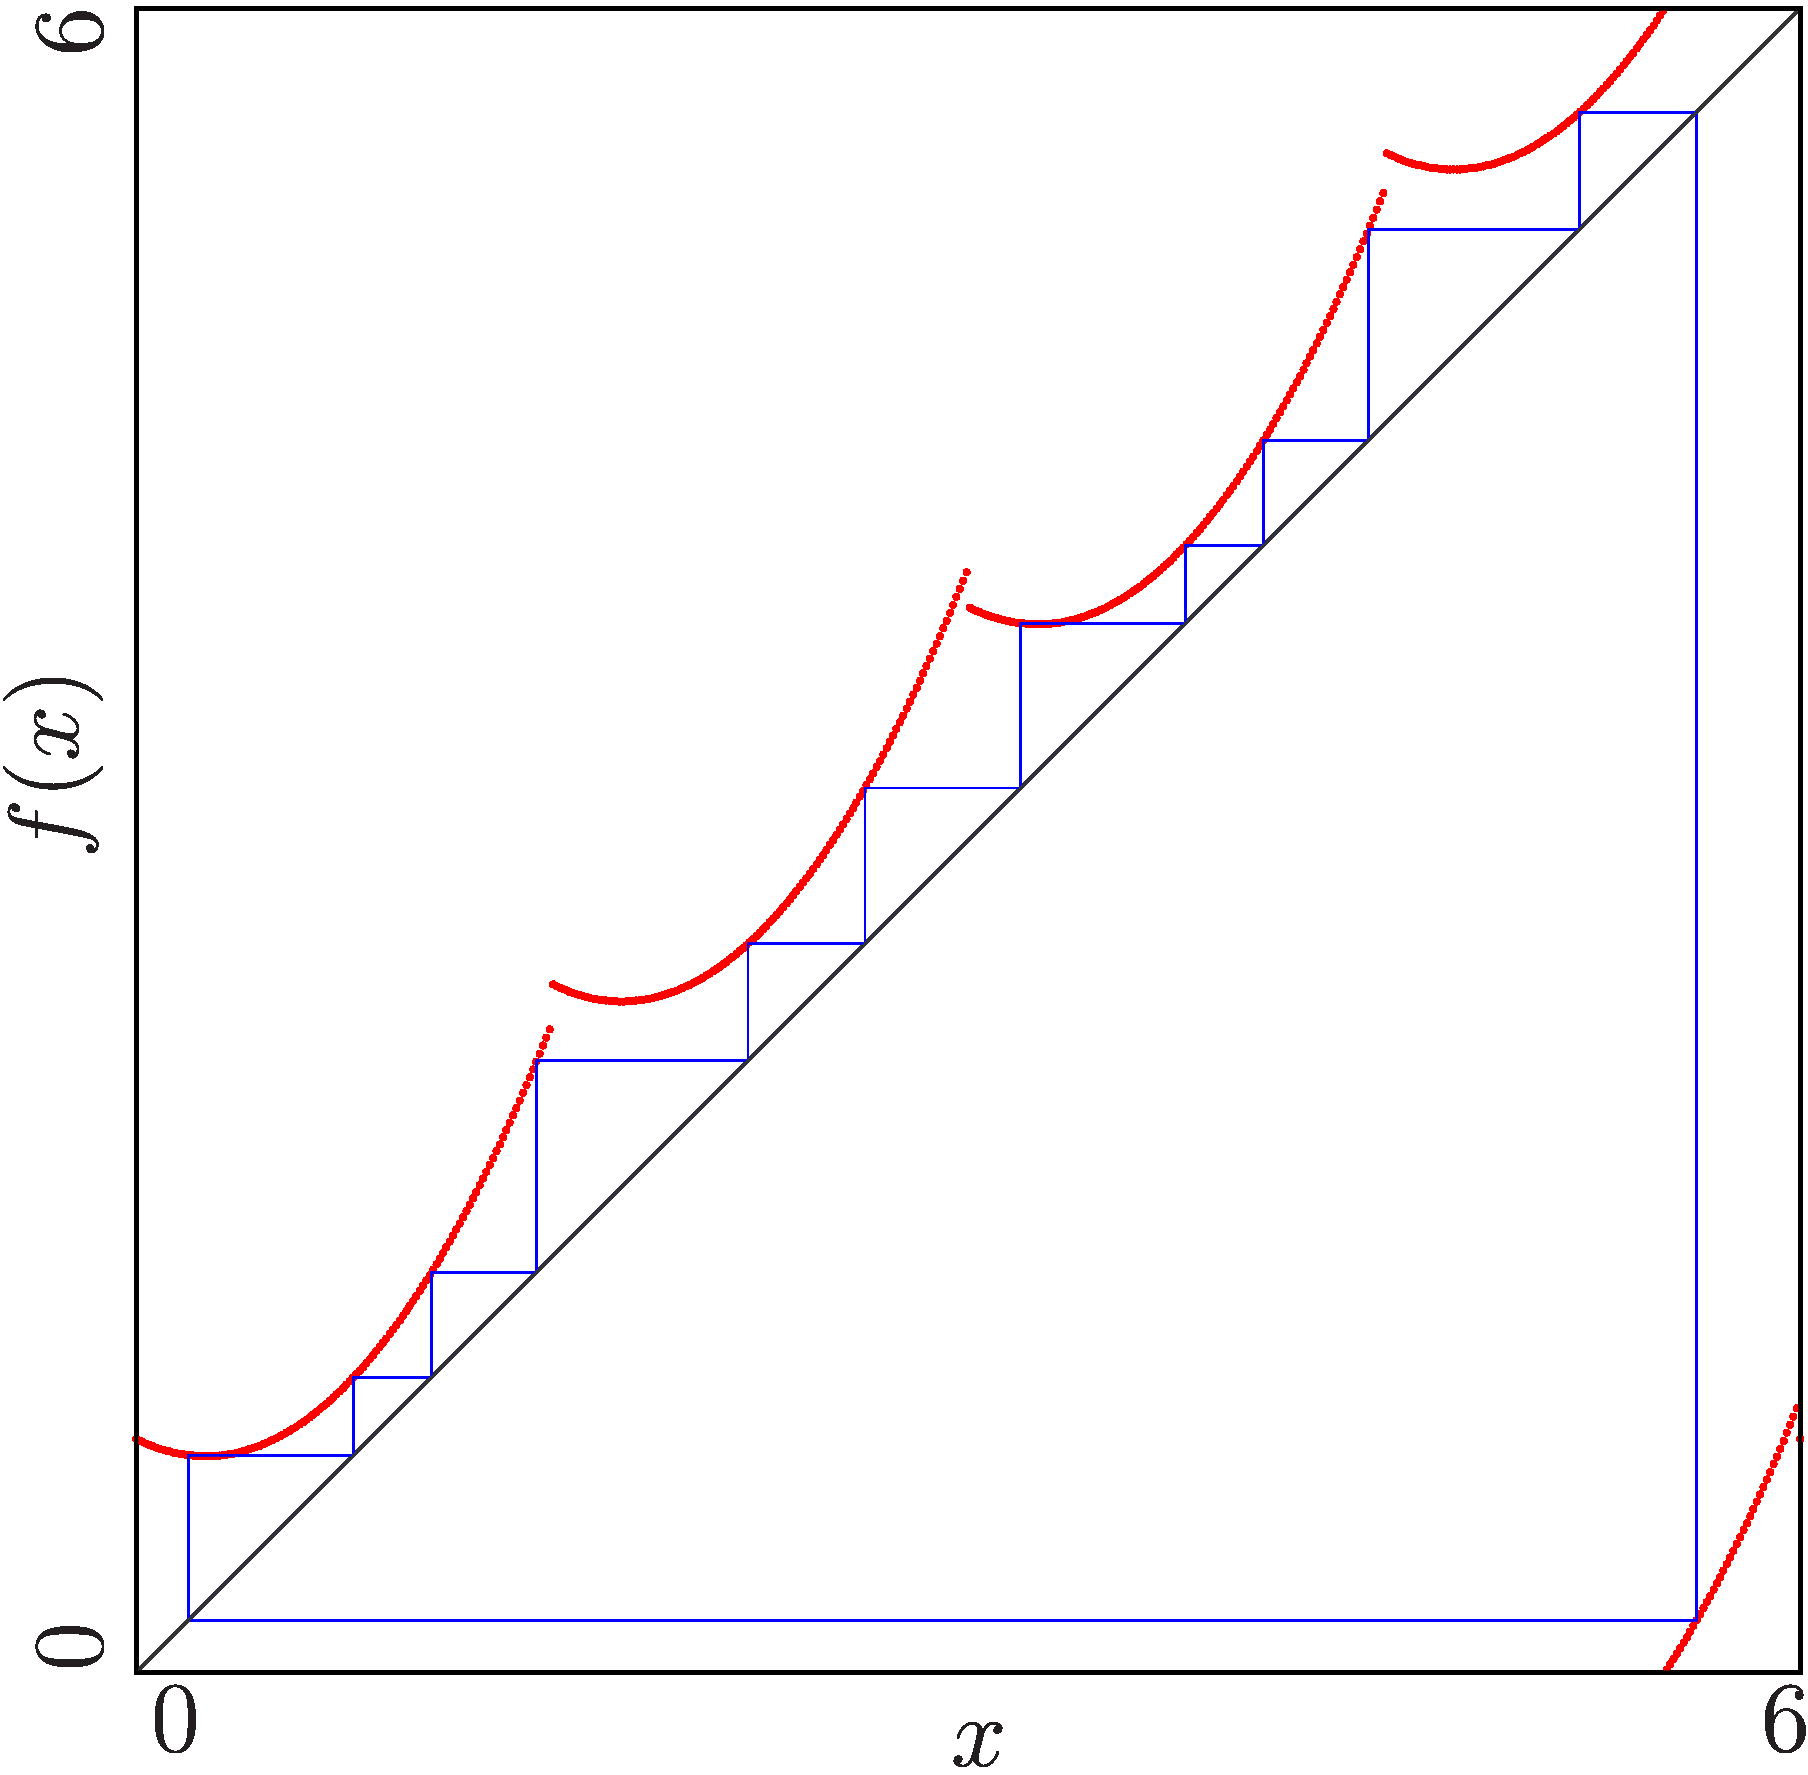
\includegraphics[width=\textwidth]{21_Quadratic_mod6/TestingDifferentParameters/cLbR/Cobweb_cLbR/result_A.png}
        \caption{Before border}
        \label{fig:quad.full.cLbR.CobwebA}
    \end{subfigure}
    \begin{subfigure}{0.3\textwidth}
        \centering
        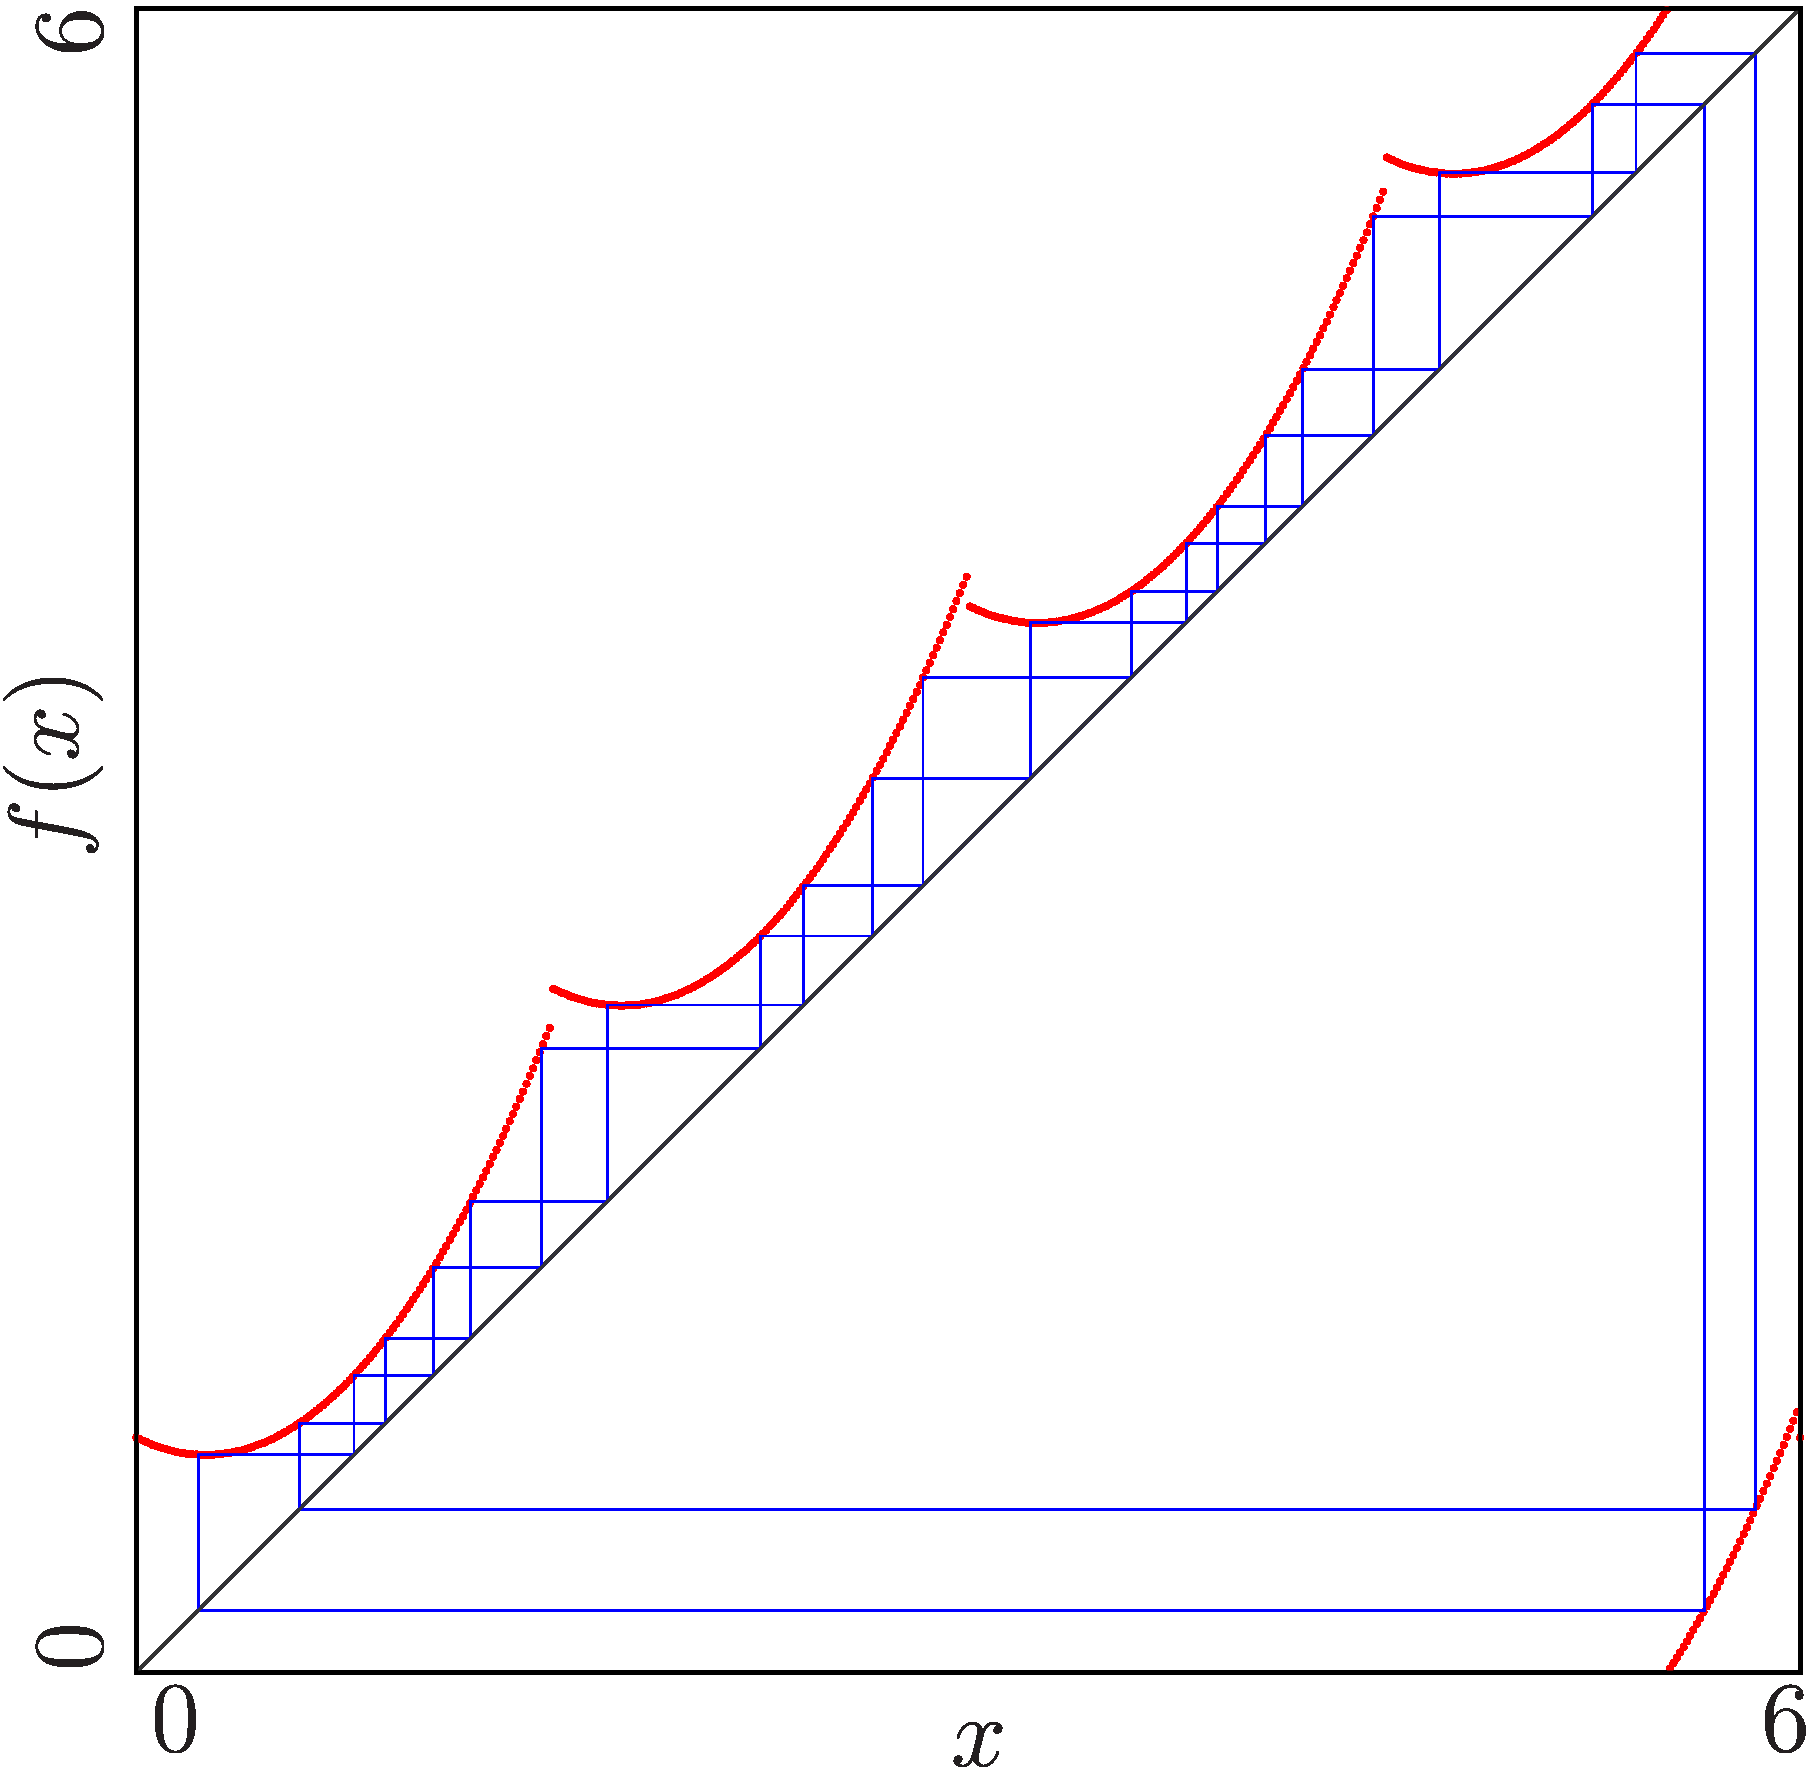
\includegraphics[width=\textwidth]{21_Quadratic_mod6/TestingDifferentParameters/cLbR/Cobweb_cLbR/result_B.png}
        \caption{At border}
        \label{fig:quad.full.cLbR.CobwebB}
    \end{subfigure}
    \begin{subfigure}{0.3\textwidth}
        \centering
        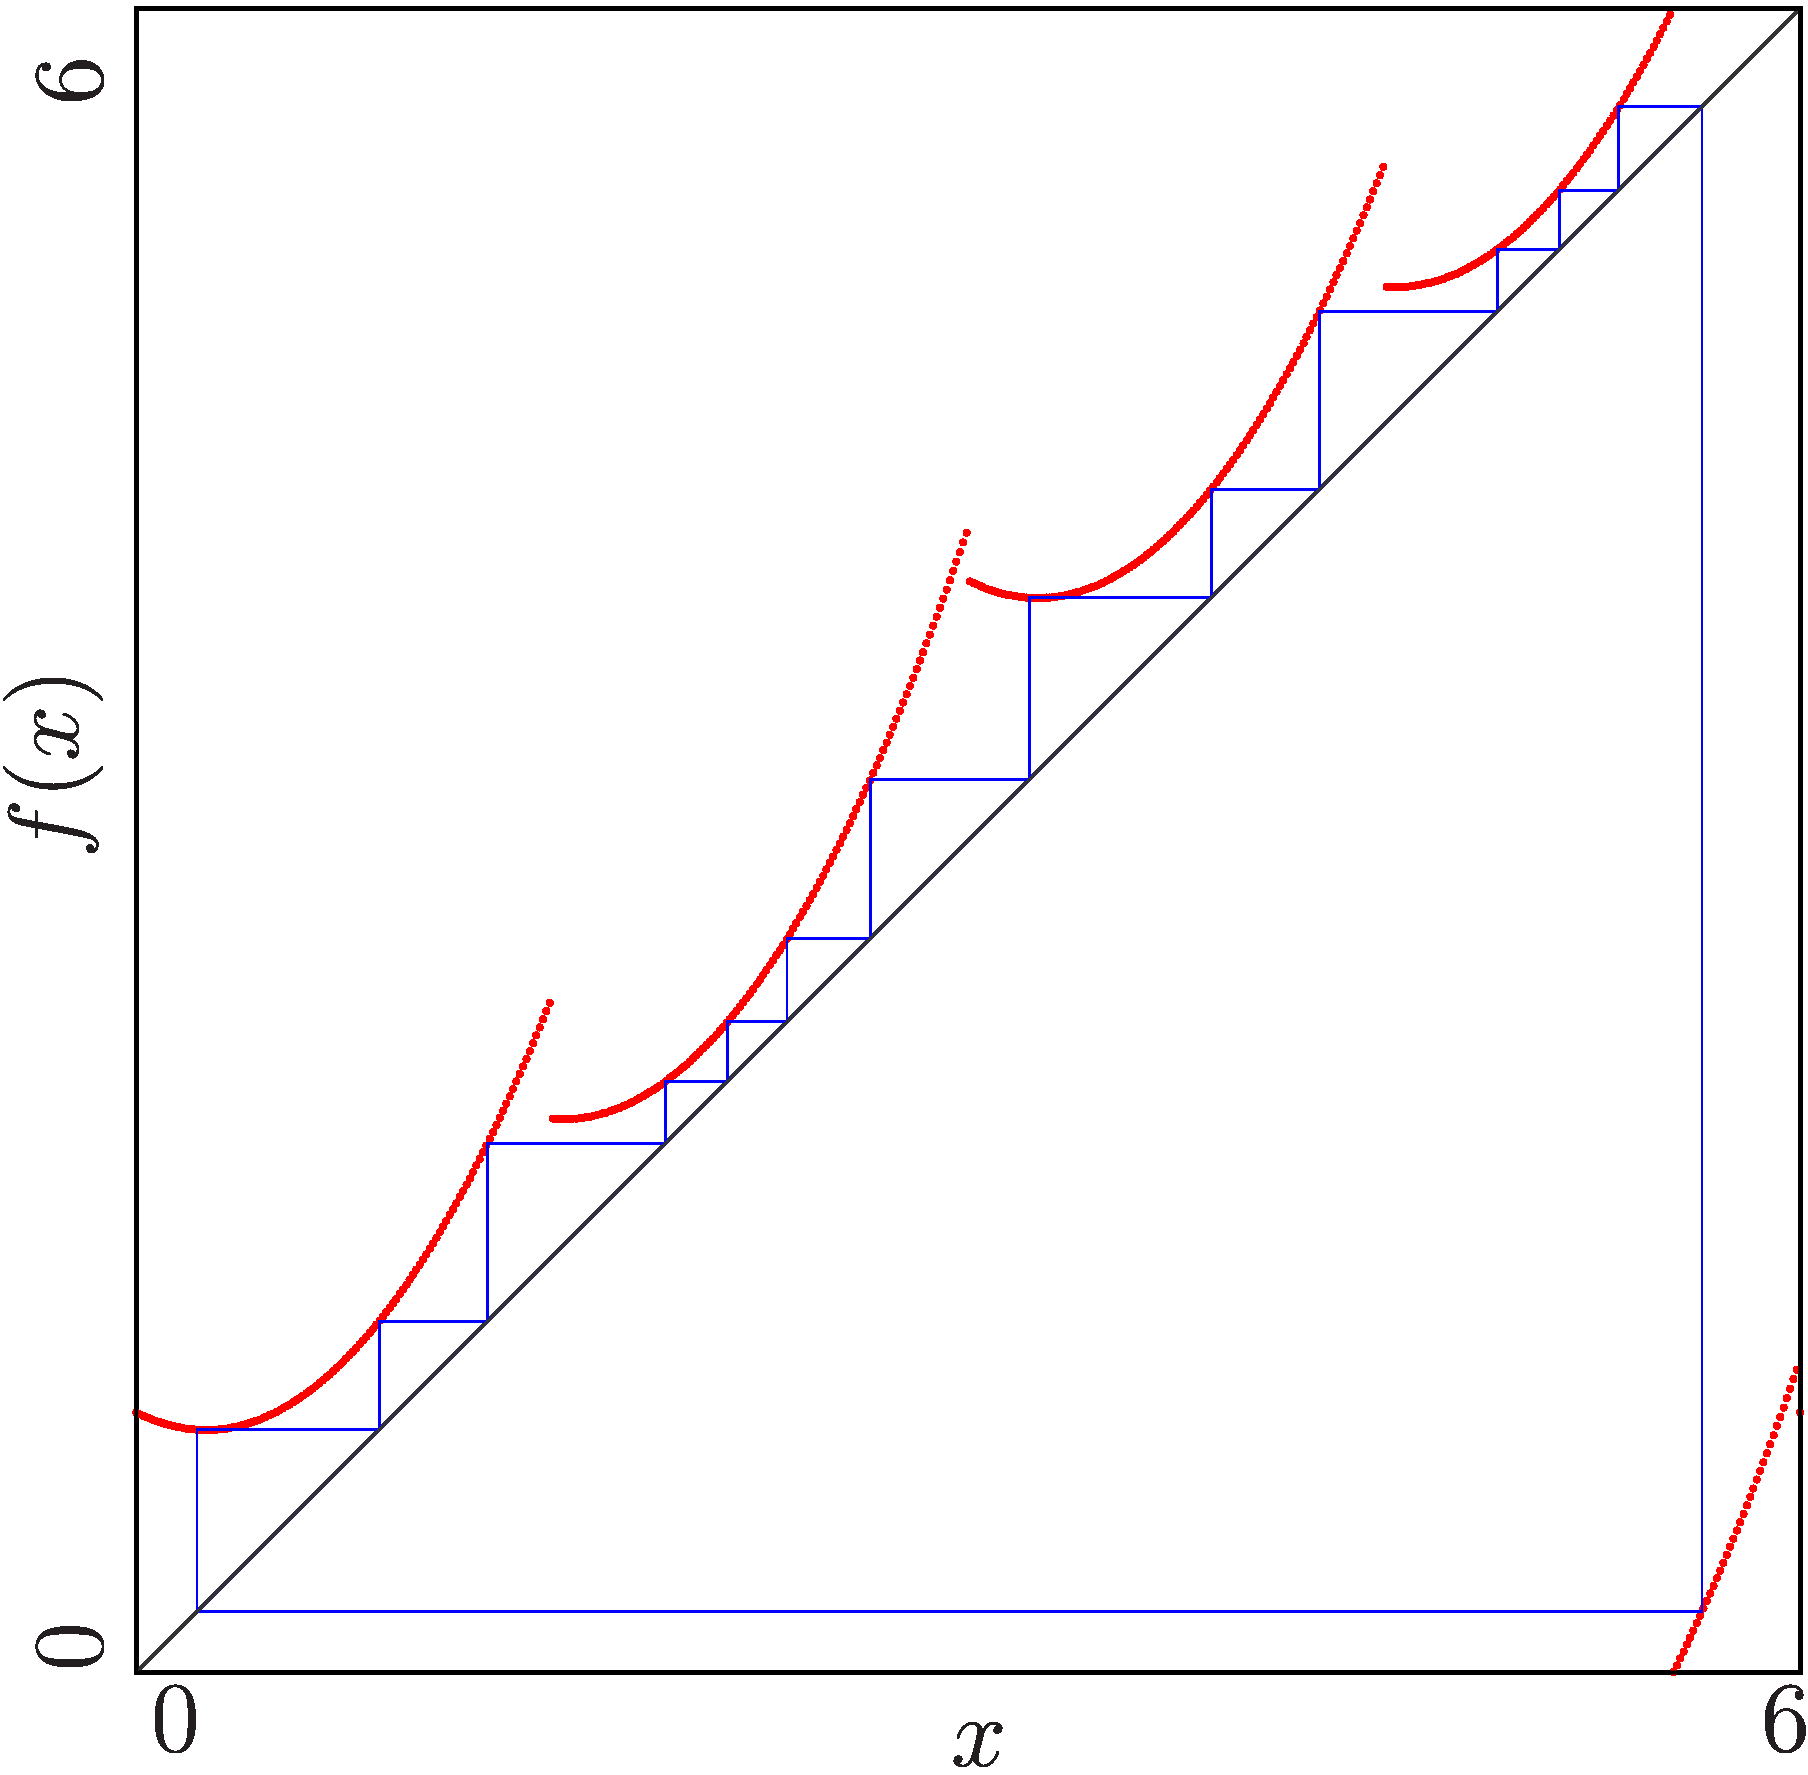
\includegraphics[width=\textwidth]{21_Quadratic_mod6/TestingDifferentParameters/cLbR/Cobweb_cLbR/result_C.png}
        \caption{After border}
        \label{fig:quad.full.cLbR.CobwebC}
    \end{subfigure}
    \caption{Cobwebs along marked line}
    \label{fig:quad.full.cLbR.Cobwebs}
\end{figure}

\subsubsection{Fixing $a_L = a_R = 1, c_L = 1.03, c_R = 2.5$}

Since varying $c_L$ in the positive direction lifts both sides of branches $\A$ and $\C$ and in the original model only the left side moves upwards, we now try to fix $c_L$ and instead vary $b_L$.
\Cref{fig:quadratic.full.bLbR.2d.full} shows a 2D scan of the behavior of cycles in this model under variation of $b_L$ and $b_R$.
\Cref{fig:quadratic.full.bLbR.2d.z} shows a zoomed-in version of that 2D scan with three points, where cobwebs are made.
In the areas containing the three points, something similar happens, to what is happening in the original model.

\begin{figure}
    \centering
    \begin{subfigure}{0.4\textwidth}
        \centering
        \includegraphics[width=\textwidth]{21_Quadratic_mod6/TestingDifferentParameters/bLbR/2D_Period_bLbR/result.png}
        \caption{Full}
        \label{fig:quadratic.full.bLbR.2d.full}
    \end{subfigure}
    \begin{subfigure}{0.4\textwidth}
        \centering
        \includegraphics[width=\textwidth]{21_Quadratic_mod6/TestingDifferentParameters/bLbR/2D_Period_bLbR_Zoomed/result.png}
        \caption{Zoomed}
        \label{fig:quadratic.full.bLbR.2d.z}
    \end{subfigure}
    \caption{2D Scan of Model Imitating the Original model \todo{choose better caption, labels different color}}
\end{figure}

The cobwebs are side by side in \Cref{fig:quad.full.bLbR.Cobwebs}.
The first cycle at point $A$, depicted in \Cref{fig:quad.full.bLbR.CobwebA}, has period 18 and its symbolic sequence is $\A^4\B^4\C^4\D^4$.
The cycle at point $C$, depicted in \Cref{fig:quad.full.bLbR.CobwebC}, has period 12 and its symbolic sequence is $\A^3\B^3\C^3\D^3$.
Thus far, what happens here has nothing to do with our original model, since the periods are different.
But in the middle, something interesting is happening.
At point $B$, two cycles are coexisting.
Note that the point was chosen lower to better illustrate the following observations, the same thing is happening in the whole area of this color.
The first one has period 14 and its symbolic sequence is $\A^4\B^4\C^3\D^3$.
And the other one also has period 14 and its symbolic sequence is $\A^3\B^3\C^4\D^4$.
This is similar to the original model because there the coexisting cycles also behaved like the one cycle on the left half of the model and like the other cycle on the right half of the model.

\begin{figure}
    \centering
    \begin{subfigure}{0.3\textwidth}
        \centering
        \includegraphics[width=\textwidth]{21_Quadratic_mod6/TestingDifferentParameters/bLbR/Cobweb_bLbR_A/result.png}
        \caption{Point A}
        \label{fig:quad.full.bLbR.CobwebA}
    \end{subfigure}
    \begin{subfigure}{0.3\textwidth}
        \centering
        \includegraphics[width=\textwidth]{21_Quadratic_mod6/TestingDifferentParameters/bLbR/Cobweb_bLbR_B/result.png}
        \caption{Point B}
        \label{fig:quad.full.bLbR.CobwebB}
    \end{subfigure}
    \begin{subfigure}{0.3\textwidth}
        \centering
        \includegraphics[width=\textwidth]{21_Quadratic_mod6/TestingDifferentParameters/bLbR/Cobweb_bLbR_C/result.png}
        \caption{Point C}
        \label{fig:quad.full.bLbR.CobwebC}
    \end{subfigure}
    \caption{Cobwebs at marked points}
    \label{fig:quad.full.bLbR.Cobwebs}
\end{figure}
